\documentclass[11pt]{scrartcl}
\usepackage[sexy]{{style_files/evan}}

\usepackage{{style_files/NMC}}
\usepackage{standalone}
\usepackage{import}

\begin{document}
\title{NMC Problem Set \#11} % add # of pset
\date{Oct. 30, 2022} % add date
\maketitle

\section*{Welcome!}

This is a selection of interesting problems derived from curious thoughts, curated so you can nibble on them throughout the week! The point of this document is to introduce you to fun puzzles that require thinking. We recommend you try the ones that you find interesting! Feel free to work on them with others (even us teachers!). Harder problems are marked with chilies (\fullchili), in case you want to challenge yourself.
\newline\newline
Have fun! \textit{Note: New variants on these problems may be released throughout the week. Remember to check back once in a while!}
    
\section{Algebra}
\begin{enumerate}[label=\textbf{A\arabic*}.]
    \item \textbf{Trig inequalities}
    \begin{enumerate}
        \item Show that $\sin(x) + \cos(x) \le \sqrt{2}$ for all real numbers $x$.
        
        \item Let $x$ and $y$ be real numbers. Show that at least one of 
        \[ \sin(x) + \cos(y) \text{ or } \sin(y) + \cos(x) \]
        is less than or equal to $\sqrt{2}$.
        
        \item Given that $x_1, x_2, x_3, ..., x_n$ are real numbers, show that at least one of 
        \[ \sin(x_1) + \cos(x_2), \sin(x_2) + \cos(x_3), \dots, \sin(x_n) + \cos(x_1) \]
        is less than or equal to $\sqrt{2}$.
    \end{enumerate}
\end{enumerate}

\newpage
\section{Combinatorics}
\begin{enumerate}[label=\textbf{C\arabic*}.]
    \item \textbf{Niko's Lightbulb Puzzle}\\
    Niko has an $N \times N$ grid of lightbulbs. In the beginning, all of the bulbs are turned off. Each move, Niko picks a row or a column. They then flip the switch for each bulb in the chosen line, lighting up unlit bulbs and vice versa. Prove that if, in any given moment, there is at least one lightbulb on, then at least $N$ lightbulbs are on in total.
\end{enumerate}

\newpage
\section{Geometry}
\begin{enumerate}[label=\textbf{G\arabic*}.]
    \item \textbf{Polygon Nesting} \newline
    \begin{enumerate} 
        \item Suppose we have a square, and we pick a point on each side. If we connect the dots together to form a quadrilateral, what's the minimum possible area it can have?
        
        \item Suppose we have a regular pentagon now. Repeating the process from earlier, what's the minimum possible area of the nested pentagon?
        
        \item (\fullchili) Generalize this problem to a regular polygon with $n$ sides.
    \end{enumerate}
\end{enumerate}

\begin{figure}[h]
        \centering
        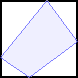
\includegraphics[width = 4cm, page=1]{weekly/week 11/Diagrams/minarea.pdf}
        \hspace{2em}
        \includegraphics[width = 4cm, page=2]{weekly/week 11/Diagrams/minarea.pdf}
        \caption{Polygons inside other polygons}
        \label{fig:minarea}
\end{figure}

\newpage
\section{Number Theory}
\begin{enumerate}[label=\textbf{N\arabic*}.]
    \item \textbf{Euler's Prime Generator} \newline
    In $1772$, Euler discovered the following function
    \[ f(n) = n^2 + n + 41 \]
    had some interesting properties. It seemed like the values $f(0), f(1), f(2), \dots$ were all prime numbers! Perhaps the function was a prime generator. Or... was Euler wasting his time? \footnote{ofc not really but yeah lol}
    
    \begin{enumerate}
        \item Can you find an example of a natural number $n$ such that $f(n)$ is not prime?

        \item Find an example of a non-constant polynomial function $f(n)$ that is \emph{never} prime for any integer value of $n$.

        \item Find an example of a non-constant polynomial such that the greatest common divisor of its coefficients is $1$.
        
        \item Show that there does not exist a non-constant polynomial $f$ such that $f(n)$ is prime for all natural numbers $n$.
        
        \item (Dirichlet, \fullchili \hspace{1pt} $\times$ 3+) \footnote{this is a joke question, it's... not a simple proof by any means. you're welcome to try though. \href{https://math.rice.edu/~av15/Files/Dirichlet.pdf}{here's a good explanation}} Prove that for any relatively prime integers $a, b$, the function $f(n) = an + b$ will be prime infinitely often.
    \end{enumerate}
\end{enumerate}
\end{document}
